\documentclass{beamer}
\usetheme{metropolis}           % Use metropolis theme
\title{\LaTeX \  und Kommunismus}
\usepackage{breqn}
\date{\today}
\author{Kimi Müller}
% \institute{Centre for Modern Beamer Themes}
\begin{document}
  \maketitle
  \section{WZF?!}
  \begin{frame}{Zwei Themen?}
    \begin{itemize}
        \item<1-> \textbf{Problem:} Ich möchte gerne über Kommunismus reden, habe aber viel Aufwand in die Präsentation gesteckt.
        \item<2-> \textbf{Lösung:} Ich referiere kurz über \LaTeX und danach über Kommunismus.
        \item<3-> \textbf{Grundlage:} Thema ist frei wählbar
        \item<4-> \textbf{Herausforderung:} unspannendes Thema spannend aufbereiten
    \end{itemize}
  \end{frame}
  \begin{frame}
    
\includegraphics[width=\textwidth]{Modern_Problems_Require_Modern_Solutions.jpg}
  \end{frame}
  \begin{frame}{Agenda}
\begin{itemize}
    \item Disclaimer
    \item Was ist \LaTeX?
    \item Warum \LaTeX?
    \item Was ist Kommunismus?
    \item Wie zwingt man jemanden zur Arbeit?
    \item Was tut die Gesellschaft, wenn man nicht hereinpasst?
\end{itemize}
  \end{frame}
  \begin{frame}{Disclaimer}
\textbf{Ich bin kein Experte in \LaTeX, Kommunismus oder Präsentationen. Ich liebe die Freiheitlich-Demokratische Grundordnung, diese Präsentation dient nur zu theoretischen und Unterhaltungszwecken.}
\end{frame}
  \section{Was ist \LaTeX?}
  \begin{frame}{WYSIWYG}
    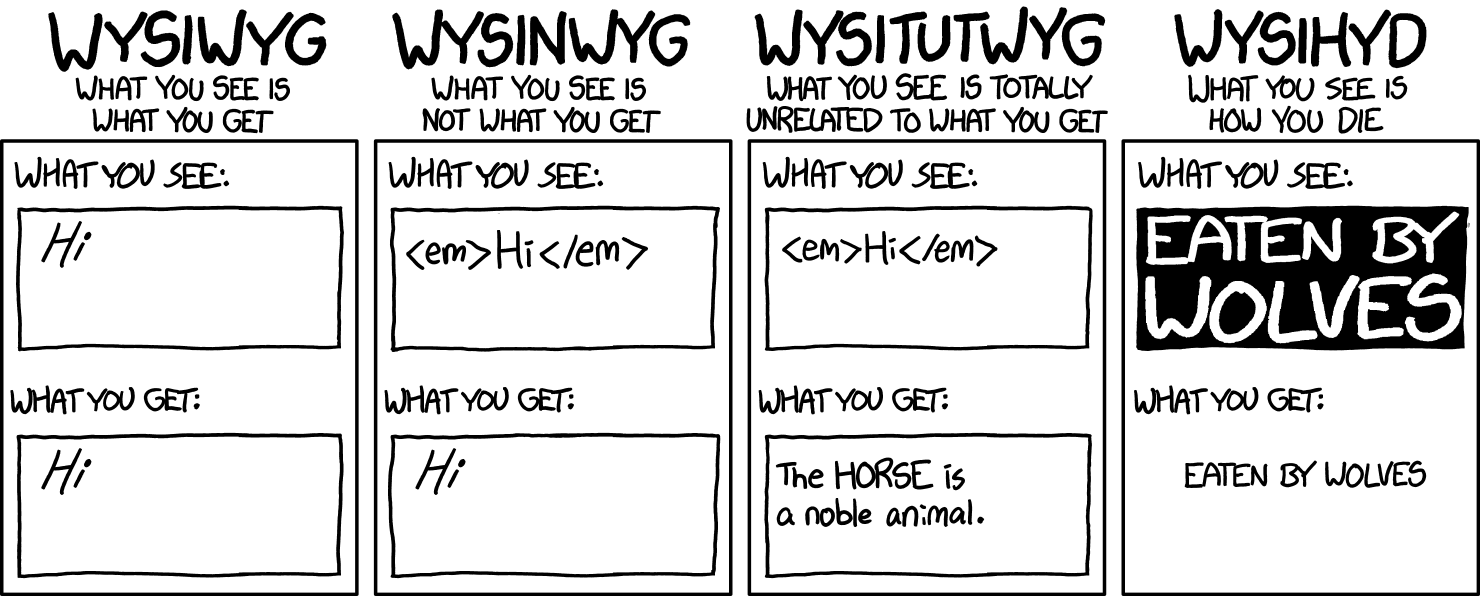
\includegraphics[width=\textwidth]{types_of_editors_2x.png}
  \end{frame}
  \begin{frame}{Echtes Beispiel dieser Präsentation}
  \end{frame}
  \section{Warum \LaTeX?}
  \begin{frame}
\begin{dmath}
  Q(\lambda,\hat{\lambda}) = -\frac{1}{2} P{(O \mid \lambda )} \sum_s \sum_m \sum_t \gamma_m^{(s)} (t) \left( n \log(2 \pi ) + \log \left| C_m^{(s)} \right| + \left( \mathbf{o}_t - \hat{\mu}_m^{(s)} \right) ^T C_m^{(s)-1} \left(\mathbf{o}_t - \hat{\mu}_m^{(s)}\right) \right)
\end{dmath}
\end{frame}
\begin{frame}{Dasselbe in Word}
\href{https://i.makeagif.com/media/5-28-2022/dXcfrH.gif}{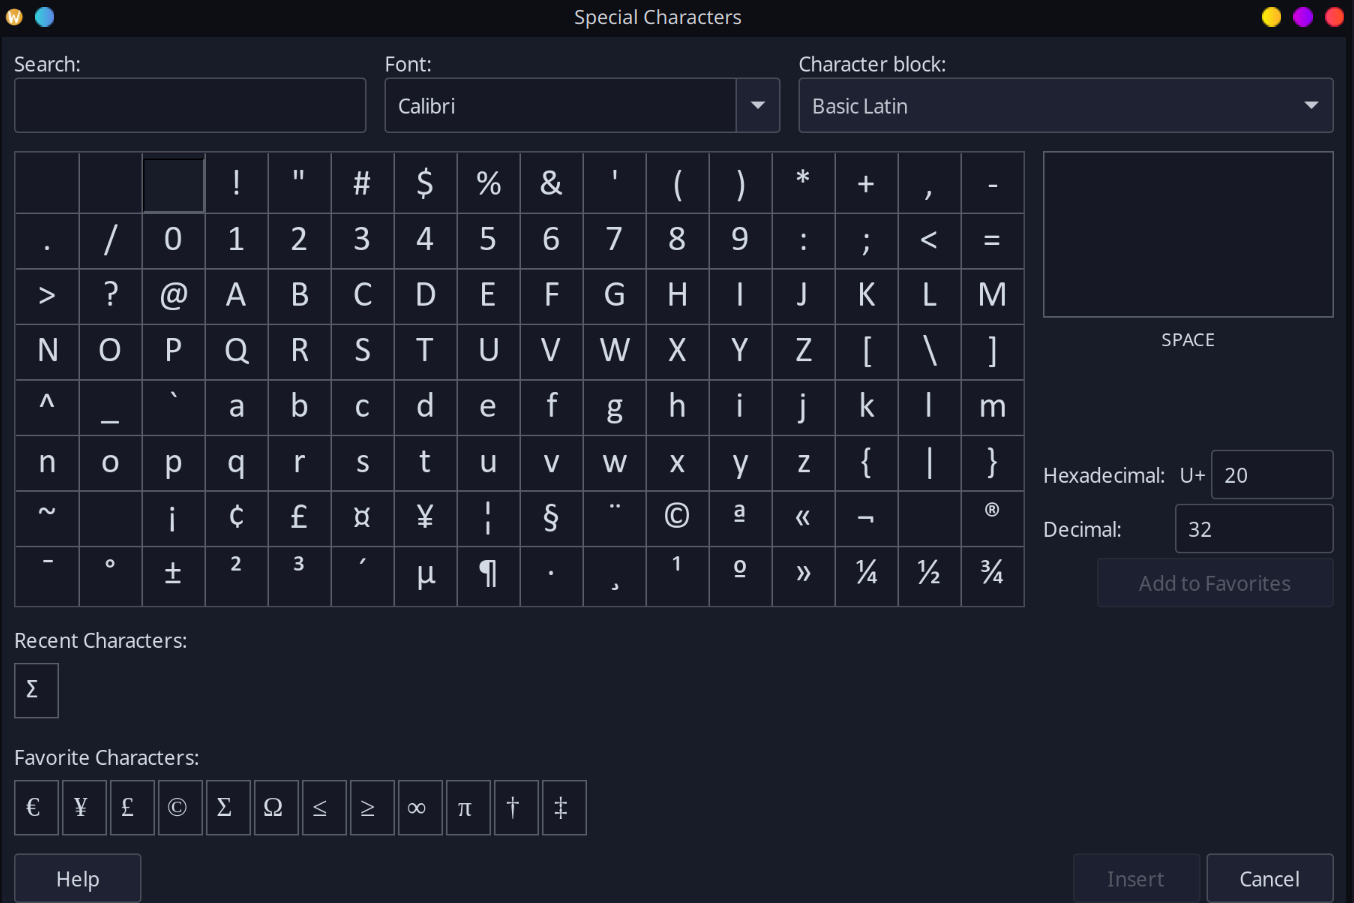
\includegraphics[width=\textwidth]{FormelnWord.png}}
\end{frame}
\begin{frame}{Link mit einsteigerfreundlichen Informationen}
\href{Link mit einsteigerfreundlichen Informationen}{https://www.overleaf.com/}
\end{frame}

\begin{frame}{Eigenschaften von \LaTeX}
    \begin{itemize}
        \item<2-> Beitrag von Vielen für Viele
        \item<3-> Große Community
        \item<4-> Komplexe Anwendung, aber simples Konzept
        \item<5-> Funktioniert besser als man denkt
        \item<6-> Belächelt von Menschen, die es nicht verstehen
    \end{itemize}

        $\Rightarrow$ auf den ersten Blick unattraktiv, aber unterschätzt.
\end{frame}

\begin{frame}{Eigenschaften von \LaTeX\ und Kommunismus}
    \begin{itemize}
        \item Beitrag von Vielen für Viele
        \item Große Community
        \item Komplexe Anwendung, aber simples Konzept
        \item Funktioniert besser als man denkt
        \item Belächelt von Menschen, die es nicht verstehen
    \end{itemize}
        $\Rightarrow$ auf den ersten Blick unattraktiv, aber unterschätzt.
\end{frame}
%\section{Kommunismus}

\begin{frame}
\section{Was  ist Kommunismus?}
\begin{itemize}
\item In dieser Präsentation: ein überspannendes Framework, um verschiedene Ansichten zusammenzufassen
\item Viele viele Details, die ich euch erspare. (Stalininisten vs Trotskisten, Histomat/Diamat, Ideologiekritik, Warenfetisch, subaltern)
\item 200 Jahre Theorien in diesem Feld in $\approx$ 6 Minuten
\end{itemize}
\end{frame}


\begin{frame}{Mehrwerttheorie - Stellt euch vor...}
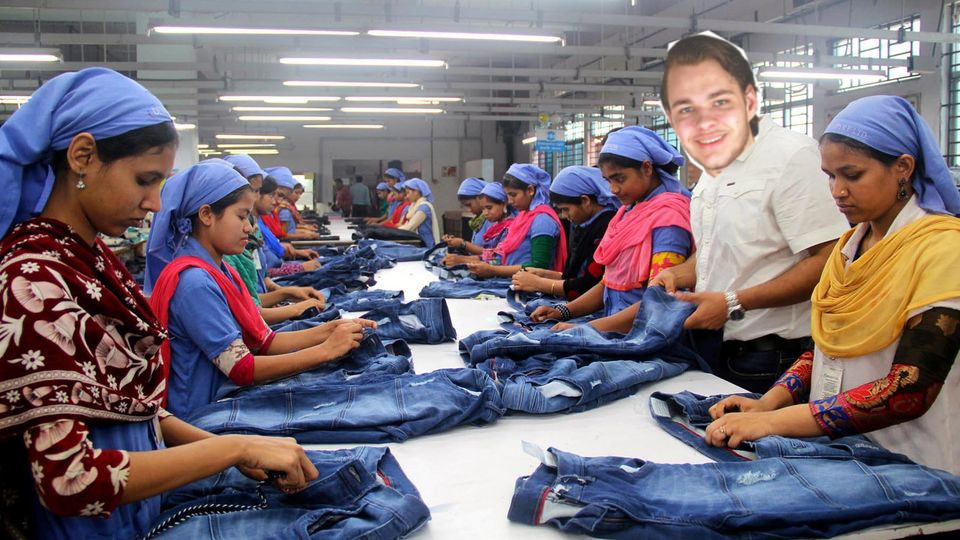
\includegraphics[width=\textwidth]{naeherinnen.jpg}
\end{frame}
\begin{frame}{Mehrwerttheorie}
\begin{itemize}
    \item \textbf{Mehrwert}: Die Arbeiter produzieren mehr Wert, als sie in Form von Löhnen zurückerhalten. Die Differenz nennt sich Mehrwert.
    \item \textbf{Akkumulation}: Der vom Arbeiter erschaffene Mehrwert wird vom Kapitalisten reinvestiert, um mehr Kapital zu akkumulieren und somit den Produktionsprozess zu erweitern.
\end{itemize}
\end{frame}
\section{Wie zwingt man Arbeiter zur Arbeit?}
\begin{frame}{Zwei Ansätze, die ineinander greifen}
\begin{itemize}
 \item Reservearmee des Kapitals
 \item Stummer Zwang der materiellen Verhältnisse
\end{itemize}
\end{frame}
\begin{frame}{Der stumme Zwang der materiellen Verhältnisse}

\includegraphics[width=0.75\linewidth]{hungern-arbeiten.jpg}
\end{frame}

\begin{frame}{Reservearmee des Kapitals}

\includegraphics[width=\linewidth]{stummer-zwang.jpg}
\end{frame}
\begin{frame}{Was tut die Gesellschaft mit Menschen, die nicht reinpassen?}
    
\includegraphics[width=\textwidth]{sexy_foucault.png}
\end{frame}
\begin{frame}{Sie überwacht und straft}
    
\includegraphics[width=\textwidth]{is_this_prison.jpeg}
\end{frame}
\begin{frame}{Danke für eure Aufmerksamkeit!}
 \href{https://www.youtube.com/watch?v=l8ukak8P2vY}{ich, wenn ich keine 1 bekomme}
\end{frame}
\end{document}
